\documentclass{ximera}
\typeout{Start loading xmPreamble.tex} %Prints message on terminal and log file. 

% Add here extra macro's that are loaded automatically by all documents of claas 'ximera' or 'xourse' in this repo 
\usepackage{tikz}
\usepackage{amsmath}
\usetikzlibrary{arrows}
\usepackage{graphicx}\usepackage{amssymb}

%\newcommand{\rulecolor}[1]{\def\CT@arc@{\color{#1}}}   %Error with Rule color when I hit serve
\definecolor{darkblue}{rgb}{0.4,0.5,0.85}
\definecolor{blue}{rgb}{0.1,0.3,.95}
%\definecolor{blue}{rgb}{0.1,0.2,0.90}
\definecolor{pink}{rgb}{0.6,0.4,0.7}
\definecolor{green}{rgb}{0.4,0.6,0.5}
\definecolor{yellow}{rgb}{0.1,0.6,0.8}
\definecolor{red}{rgb}{0.8,0.1,0.5}
\definecolor{glaucous}{rgb}{0.38,0.51,0.71}

\usepackage{pgfplots}
\pgfplotsset{compat=1.16}
\usetikzlibrary{calc,angles,positioning,intersections,quotes,decorations.markings}
\pgfplotsset{soldot/.style={only marks,mark=*, line width=0.2pt, mark size=1.5pt}}
\pgfplotsset{holdot/.style={fill=white,only marks,mark=*, line width=1.0pt, mark size=1.5pt}}


\usepackage[utf8]{inputenc}  %needed to define \begin{axis} in tikz pic

%%
%%  Example:
%%
% \newcommand{\R}{\mathbb{R}


\title{Collection of Activities}
\author{Kelly Stady}

\begin{document}
\begin{abstract}
    Practice Problems
\end{abstract}
\maketitle


\begin{question}
    $2+3=\answer{5}$
\end{question}


\begin{question}
    The circle below has been divided into 10 equal parts.  What fraction of the circle is shaded?
   
    \bigskip

   %\begin{image}  %Makes circle huge!!  scale=0.1 does not help
   \hspace{0.8in} 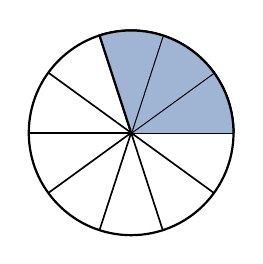
\begin{tikzpicture}
   \draw[thick] (0,0) circle [radius=1.3cm];
   \foreach \i in {36,72,...,360}
    \draw[semithick] (0,0)--(\i:1.3cm);    %The colon signifies that polar coordinates are being used. (60:.75cm) means the point that is at an angle of 60° and a distance of 0.75cm from the origin. Length of radial lines - should match radius above.
    \draw[thick, fill=glaucous!60] (0,0) --  (36:1.3) arc(36:0:1.3); %To Draw Arc: \draw (x,y) arc (start:stop:radius);
    \draw[thick, fill=glaucous!60] (0,0) --  (72:1.3) arc(72:36:1.3); %Colon indicates polar coordintes (angle:length)
    \draw[thick, fill=glaucous!60] (0,0) --  (108:1.3) arc(108:72:1.3);
    %\draw[fill=glaucous] (0,0) -- (360:1.5) arc(360:324:1.5);
   
   \end{tikzpicture}
   %\end{image}
   
   \begin{multipleChoice}
   \choice[correct]{$\displaystyle \frac{3}{10}$}

   \choice{$\displaystyle \frac{1}{10}$}

   \choice{$\displaystyle \frac{7}{10}$}
   \end{multipleChoice}
   
   \end{question}
   


%\begin{center} %% Image is found in xmPictures
%
\includegraphics{missionPatch.jpg}
%\end{center}


\end{document}
